\section{Results}
As mentioned above, we tried 2 types of representation and have chosen to do each learning session in increments of 1,000 episodes starting from 1,000 episodes to 10,000 episodes. This was to track the progress of the algorithms and to see if there were any learning trends.
The results for them will be shown below. 

\subsection{Simple Representation}
The results from 10,000 episodes of the simple representation is shown below.

\begin{figure}[h]
	\centering
	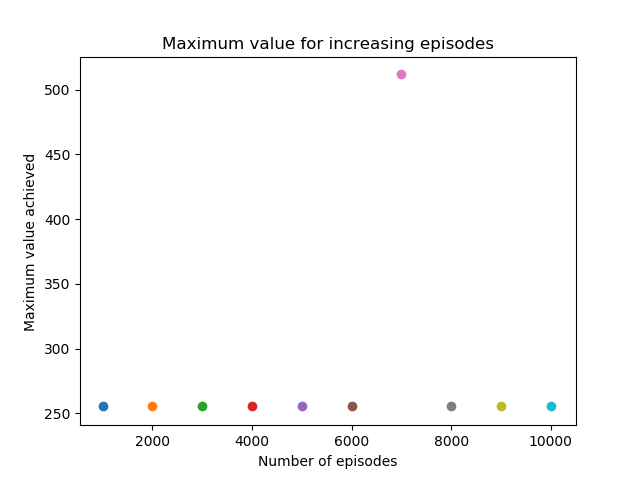
\includegraphics[width=4.0in]{experiment1}
	\caption{Results from simple representation with increasing episodes}
	\label{fig:experiment1}
\end{figure}

From the results shown in figure \ref{fig:experiment1}, it can clearly be seen that this representation is not very effective at making our agent learn how to play 2048. However, the agent was able to reach the 256 tile quickly and consistently, which could mean that the agent was either able to visit the earlier states more often, therefore getting more accurate q-values for certain states and actions, or simply chose lucky actions. Furthermore, reaching the 512 tile only once out of 10 increasing episodes shows that the tile was reached with a high level of luck rather than knowledge of the action. We have two main reasons to believe why this representation was not capable of teaching the agent 2048. The first one being that the representation did not have enough information on how the tiles relate to each other, thus not allowing the agent to choose actions based on the certain factors of the board. The second one being that there are too many combination of states and that the agent was not able to visit all the states in the amount of episodes provided. 

\subsection{Relationship Representation}
The results from 10,000 episodes of the relationship representation is shown below.
\\

\begin{figure}[h]
	\centering
	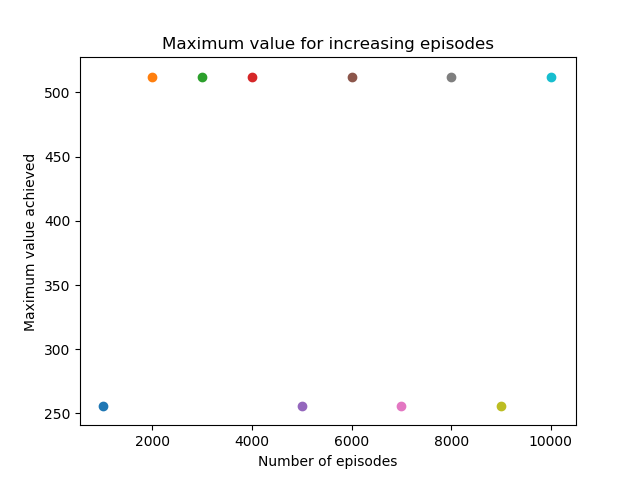
\includegraphics[width=4.0in]{experiment2}
	\caption{Results from relationship representation with increasing episodes}
	\label{fig:experiment2}
\end{figure}

The results from figure \ref{fig:experiment1} show that this representation is evidently more effective in learning 2048 compared to the previous representation, given the fact that it was able to reach the 512 tile with less training episodes and more consistently. However, it can also be seen that the maximum value achieved by this representation is the same as the previous representation, demonstrating that this representation was also not able to effectively teach the agent 2048. We believe that adding additional information such as interaction between tiles in the state vector has improved both the learning rate and consistency of the agent. However, the problem mentioned in the previous experiment still remains. This representation is still not able to account for the fact that there will be an impossibly large amount of unique states for the agents to visit, implying that the agent may not be able to visit every state in a feasible amount of time. 
On the other hand, it could be argued that there was not enough training time for the agent to completely learn 2048.

Moreover, it has been clear that the problem might not solely lie in the representation. The game's heavy involvement with randomness might also add complication and thus 'error' to our learning.
